
\chapter{نمونه هایی  از کدهای لاتک جهت آموزش}\label{chapter1}
\paragraphfootnotes


مشتق‌ به طور گسترده در علوم پایه، اقتصاد، پزشکی و علوم کامپیوتر\index{علوم کامپیوتر} برای محاسبه سرعت اولیه\index{سرعت اولیه} و شتاب\index{شتاب} و به
به منظور توضیح رفتار ماشین‌آلات، تخمین میزان افت آب در هنگام پمپ شدن آب از تانکر آب و پیشگویی\index{پیشگویی} نتایج ایجاد خطا در اندازه‌گیری‌ها به کار می‌رود. پیدا کردن مشتق‌ها می‌تواند طولانی و سخت باشد. می‌توان گفت مشتق یکی از ارکان اصلی حساب
دیفرانسیل\index{حساب دیفرانسیل} و انتگرال محسوب می‌شود. در این فصل، تکنیک‌هایی
برای محاسبه آسان‌تر آن‌ها بیان می‌شود.%
\cite{george95}
\section{یادآوری حدهای یک‌طرفه و کاربرد آن‌ها}
در این بخش ابتدا حدهای یک‌طرفه\index{حد!یک‌طرفه} را یادآوری کرده و بعد از آن، به بیان مفهوم مشتق\index{مشتق} می‌پردازیم. سپس روابط و
قضایای مشتق‌گیری را بیان می‌کنیم.
در تعریف 
$\lim_{x\rightarrow a}f(x)$،
$x$هایی
را در نظر می‌گیریم که در یک بازهٔ باز شامل $a$ و نه خود $a$ باشند؛ یعنی مقادیر $x$ نزدیک به $a$ را، 
چه بزرگ‌تر از $a$ باشند و چه کوچک‌تر از آن باشند. 

حال فرض کنید تابعی مانند $f(x)=\sqrt{x-4}$ داریم. چون برای
$x<4$،
مقدار $f(x)$ وجود ندارد، بنابراین $f$ در هیچ بازهٔ باز شامل $4$ تعریف نشده است. لذا 
$\lim_{x\rightarrow 4}\sqrt{x-4}$
بی‌معنی است. از آنجایی که استفاده از تعریف مشتق برای مشتق‌گیری از توابع، کاری زمان‌بر است، در این بخش، قضایایی 
را مطرح می‌کنیم که با کمک آن‌ها بتوان مشتق توابع را به سادگی به دست آورد.  شکل \ref{fig1-1} را ببینید که در آن، ناحیهٔ محصور بین نمودار $y=2-x^2$ و خط $y=-x$ را
نشان می‌دهد.

\begin{figure}[!h]
\centering
\begin{tikzpicture}[line cap=round,line join=round,>=triangle 45,x=1.0cm,y=1.0cm,]
\draw[>=latex,->,color=black,] (-1.5,0) -- (3.5,0);
\foreach \x in {-1,-1,1,2,3}
\draw[shift={(\x,0)},color=black] (0pt,2pt) -- (0pt,-2pt) node[below] {\footnotesize $\x$};
\draw[>=latex,->,color=black] (0,-2.5) -- (0,3);
\foreach \y in {-2,-1,1,2,2.5}
\draw[shift={(0,\y)},color=black] (2pt,0pt) -- (-2pt,0pt);
\draw[color=black] (0pt,-1pt) node[below left] {\footnotesize $0$};
\node at (-1,1) [left ] {\small $(-1,1)$};
\node at (3.5,0) [right ] {\small $x$};
\node at (0,3) [above ] {\small $y$};
\clip[] (-1.5,-2.5) rectangle (3.5,3);
\draw [very thick,domain=-1.5:2.5] plot(\x,{-1*(\x)});
\draw [smooth, very thick,domain=-2:3] plot(\x,{-1*(\x)^2+2});
\node at (2,-2) [right] {\small $(2,-2)$};
\node at (.7,-1.2) [below ] {\small $y=-x$};
\node at (1,1) [right ] {\small $y=2-x^2$};
\draw [fill=cyan,fill opacity=0.3] plot [domain=-1:2](\x,{-1*(\x)^2+2}) -- plot [domain=-2:3] (\x,{-1*(\x)});
\end{tikzpicture}
\caption{ناحیهٔ محصور ایجاد شده توسط سهمی $y=2-x^2$ و خط $y=-x$}
\label{fig1-1}
\end{figure}

 با وجود این، اگر $x$ را فقط به مقادیر بزرگ‌تر از $4$ محدود کنیم، می‌توانیم مقدار $\sqrt{x-4}$
را به اندازهٔ دلخواه به $0$ نزدیک کنیم؛ 
%با شرط اینکه $x$ها را بزرگ‌تر از $4$ ولی به اندازهٔ کافی نزدیک به $4$ بگیریم.
در چنین حالتی، $x$ را از سمت راست به $4$ میل می‌دهیم و آن‌را حد یک‌طرفه از راست و یا حد راست\index{حد!راست} می‌نامیم. بنابراین
\[
\lim_{x\rightarrow 4^{+}}\sqrt{x-4}=0.
\]
حد چپ\index{حد!چپ} نیز به صورت مشابه تعریف می‌شود.


اگر تابع $f$ در $x_1$ تعریف شده باشد، آنگاه مشتق راست $f$ در $x_1$ با $f'_{+}(x_1)$ 
\psymbol{$f'_{+}(x)$}{مشتق راست  $f$ در نقطهٔ $x$}
نشان داده می‌شود و به صورت 
\begin{align}
f'_{+}(x_1)=\lim_{\Delta x\rightarrow 0^{+}}\dfrac{f(x_1+\Delta x) - f(x_1)}{\Delta x}
\end{align}
و یا به عبارت دیگر،
تعریف می‌شود؛ به شرطی که این حدود موجود باشند.
در ادامه، چند قضیه و مثال بیان می‌شود تا خواننده بیشتر با مفاهیم حد و مشتق آشنا
شود. برای بحث بیشتر می‌توان به کتاب‌های پیشرفته‌تر حساب دیفرانسیل مراجعه کرد. 

\begin{ptheorem1}[وجود حد]\label{bth1}
گوییم $\lim_{x\rightarrow a}f(x)$ وجود دارد و برابر $L$ است،  اگر و تنها اگر 
\[
\lim_{x\rightarrow a^{+}}f(x),\qquad \lim_{x\rightarrow a^{-}}f(x)
\]
هر دو موجود و برابر با $L$ باشند.
\end{ptheorem1}

\begin{example}
فرض کنید تابع $f$ مطابق شکل \ref{fig1-2} 
و با ضابطهٔ
\[
f(x)=\left\{\begin{array}{ll}
-1 & x<0\\
0 & x=0\\
1 & x>0
\end{array} \right.
\]
تعریف شده است. آیا حد%
\RTLfootnote{در ادامه فرض می‌شود خواننده تا حدودی با مفاهیم پایه‌ای حد آشناست.}
  تابع $f$ وجود دارد؟
\end{example}
\begin{figure}[!h]
\centering
\begin{tikzpicture}[line cap=round,line join=round,>=triangle 45,x=2cm,y=2cm,]
\draw[>=latex,->,color=black] (-.2,0) -- (2.3,0);
\foreach \x in {1,2}
\draw[shift={(\x,0)},color=black] (0pt,2pt) -- (0pt,-2pt) node[below] {\footnotesize $\x$};
\draw[>=latex,->,color=black] (0,-0.3) -- (0,1.5);
\foreach \y in {1}
\draw[shift={(0,\y)},color=black] (2pt,0pt) -- (-2pt,0pt) node[left] {\footnotesize $\y$};
\draw[color=black] (0pt,-5pt) node[left] {\footnotesize $0$};
\node at (.8,1.1) [below] { $y=\Big(\dfrac{x}{2}\Big)^{2/3}$};
\node at (2,.95) [ below] { $(2,1)$};
\node at (2.3,0) [right] {\small $x$};
\node at (0,1.5) [above] {\small $y$};
\draw[cyan,thick, smooth,samples=5.5*\sqrtsamples,domain=0.001:2]plot(\x,{exp(2*ln(\x/2)/3)});
\draw [fill=cyan](2,1) circle (.7mm);
\end{tikzpicture}
\caption{نمودار تابع  $y=({x}/{2})^{2/3}$ در بازه $[0,2]$}
\label{fig1-2}
\end{figure}
\begin{solution}
با توجه به تعریف تابع، اگر $x$ عددی کوچک‌تر از $0$ باشد، $f(x)$ دارای مقدار ثابت $-1$ است. لذا
$\lim_{x\rightarrow 0^{-}} f(x)=-1$.
با استدلالی مشابه، نتیجه می‌شود که 
$$\lim_{x\rightarrow 0^{+}} f(x)=+1.$$
بنابراین
\[
\lim_{x\rightarrow 0^{-}} f(x)\neq \lim_{x\rightarrow 0^{+}} f(x)
\]
و لذا حل مثال به پایان می‌رسد.
\end{solution}
\paragraphfootnotes

در معنی شناسی نمادین، برنامه‌ها و قطعه‌برنامه‌ها، به عنصرهایی از ساختارهای ریاضی مانند دامنه‌ها از دیدگاه اسکات\LTRfootnote{Scott} نگاشته می‌شود. اگر سیستم مدل‌بندی شده توانایی ایجاد انتخاب‌های تصادفی (یا انتخاب‌های 
شبه تصادفی) را داشته باشد، آنگاه منطقی است که رفتار خود را به وسیله اندازه‌ای که احتمال را برای سیستم ثبت
 می‌کند، مدل‌بندی کند تا زیرمجموعه‌ اندازه‌پذیری از مجموعه همه حالت‌های ممکن بشود. این ایده‌ها برای اولین بار توسط صاحب ‌جهرمی\LTRfootnote{Saheb-Djahromi} و کازن\LTRfootnote{Kozen}
مطرح شد. هنگامی که کازن با فضاهای اندازه مطلق کار می‌کرد، اندازه‌های (احتمال) در نظر گرفته شده قبلی، به وسیله مجموعه‌های اسکات-باز یک \lr{dcpo} گسترش پیدا کرد.

 این ارتباط بین محاسبه‌پذیری و توپولوژی، بطور بسیار واضح توسط اسمیت\LTRfootnote{Smyth}  شرح داده شده و  بعدها توسط آبرامسکی\LTRfootnote{Abramsky}، ویکرز\LTRfootnote{Vickers} و دیگران، بیشتر توسعه داده شد.

\begin{pdefinition1}[مشتق تابع]
مشتق\index{مشتق} تابع $f$، تابعی است که با علامت $f'$ نشان داده می‌شود و مقدار آن در هر عدد $x$ واقع در دامنهٔ $f$
به صورت 
\begin{align}\label{bderi1}
f'(x)=\lim_{\Delta x\rightarrow 0}\dfrac{f(x+\Delta x) - f(x)}{\Delta x}
\end{align}
\psymbol{$f'(x)$}{مشتق تابع $f$ در نقطهٔ $x$}
تعریف می‌شود؛ به شرطی که حد فوق وجود داشته باشد. شکل \ref{fig1-3} را ببینید.
\end{pdefinition1}

\begin{figure}[!h]
\centering
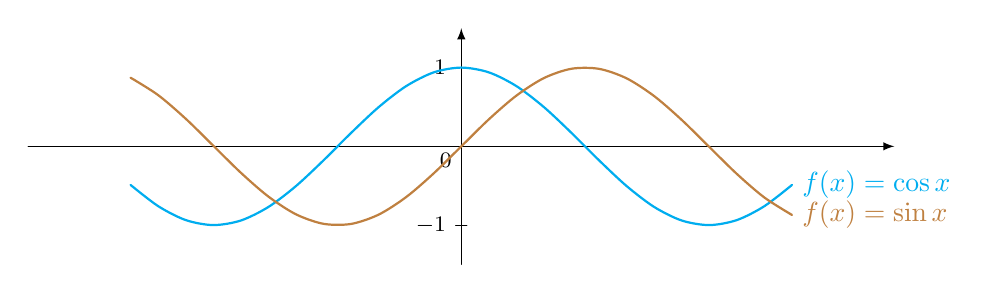
\begin{tikzpicture}[line cap=round,line join=round,]
\draw[>=latex,->,color=black] (-5.5,0) -- (5.5,0);
\foreach \x in {}
\draw[shift={(\x,0)},color=black] (0pt,2pt) -- (0pt,-2pt) node[below] {\footnotesize $\x$};
\draw[>=latex,->,color=black] (0,-1.5) -- (0,1.5);
\foreach \y in {1,-1}
\draw[shift={(0,\y)},color=black] (2pt,0pt) -- (-2pt,0pt) node[left] {\footnotesize $\y$};
\draw[color=black] (0pt,-5pt) node[left] {\footnotesize $0$};
\draw[color=cyan,smooth,thick] plot[domain=-4.2:4.2] (\x,{cos(\x r)}) node[right] {$f(x) = \cos x$};
\draw[color=brown,smooth,thick] plot[domain=-4.2:4.2] (\x,{sin(\x r)}) node[right] {$f(x) = \sin x$};
\end{tikzpicture}
%\end{tikzpicture}
\caption{نمودار دو تابع مثلثاتی $y=\sin x$ و $y=\cos x$}
\label{fig1-3}
\end{figure}

\section{انتگرال معین و نامعین و کاربرد آن در مهندسی}
در این بخش،  مفهوم انتگرال‌های معین و نامعین را توضیح داده
 و سپس خواص انتگرال معین بیان می‌شود. همچنین بعضی از کاربردهای انتگرال
 معین توضیح داده می‌شود. بعد از آن، نوبت به انتگرال‌های نامعین 
می‌رسد و روش‌های انتگرال‌گیری برای این نوع انتگرال‌ها شرح داده می‌شود.
از این روش‌ها بعدها در درس معادلات دیفرانسیل نیز استفاده می‌شود.

\subsection{انتگرال معین}
\index{انتگرال!معین}
فرض کنید $y=f(x)$ یک تابع پیوسته\index{تابع پیوسته} روی بازهٔ $[a,b]$ باشد. این بازه را به $n$ زیربازه با انتخاب $n-1$ نقطه مانند $x_1$، $x_2$، $\ldots$، $x_{n-1}$ بین $a$ و $b$ تقسیم می‌کنیم
به شرطی که 
\[
a<x_1<x_2<\cdots<x_{n-1}<b.
\]
برای ایجاد یکنواختی، $a$ را با $x_0$ و $b$ را با $x_n$ نشان می‌دهیم. شکل \ref{fig1-4} را ببینید.



\begin{theorem}[قضیه مقدار میانگین برای انتگرال‌های معین]\label{gmean}
اگر $f$ روی $[a,b]$ پیوسته باشد، آنگاه یک $c$ای در بازهٔ $[a,b]$
وجود دارد به طوری که
\[
f(c)=\dfrac{1}{b-a}\int _a ^b f(x) dx.
\]
\end{theorem}


ناحیه ممکن است  دارای شکل خاصی باشد که در این صورت، با استفاده از فرمول‌های  هندسه \cite{folland} می‌توانیم مساحت\index{مساحت} آن‌را حساب کنیم.

اگر $f$ و $g$ توابع پیوسته‌ای روی بازهٔ  $[a,b]$ و با شرط $f(x)\geq g(x)$ باشند،
آنگاه مساحت ناحیهٔ  بین منحنی‌های $y=f(x)$ و $y=g(x)$ از $a$ تا $b$ برابر است با
\begin{align}\label{ibet1}
A=\int_a^b [f(x)-g(x)] dx.
\end{align}
\subsection{منحنی‌های قاطع یکدیگر}
وقتی ناحیه‌ای توسط منحنی‌هایی که یکدیگر را قطع می‌کنند، مشخص می‌شود، 
نقاط تقاطع\index{نقاط تقاطع}، حدود انتگرال‌گیری را تعیین می‌کنند. مثال بعدی، نمونه‌ای از این 
حالت را نشان می‌دهد. در فصل بعدی باز هم نمونه‌های دیگری را بررسی خواهیم کرد که باعث فهم
بیشتر مبحث خواهد شد.


\begin{figure}[!t]
\centering
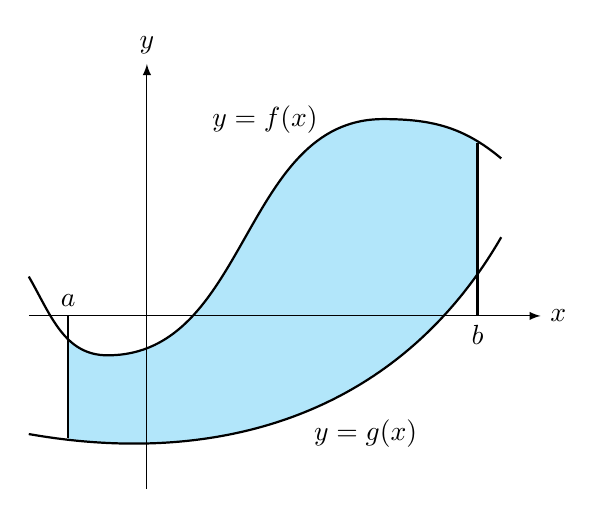
\begin{tikzpicture}[]
\begin{scope}
\clip(-1,-2)rectangle(4.2,3);
\clip (-1.5,.5) to [out=300,in=180] (-.5,-.5)
to [out=0,in=180] (3,2.5)
to [out=360,in=140] (4.5,2) --++(0,-5)--(-1,-5)--cycle;
\fill[fill=cyan,fill opacity=0.3] (-1.5,-1.5) to [out=350,in=240] (4.5,1)--++(0,5)--(-1,5)--cycle;
\end{scope}
\draw [->,>=latex] (-1.5,0) -- (5,0) node [right] {$x$};
\draw [->,>=latex] (0,-2.2) -- (0,3.2) node [above] {$y$};
\draw[thick] (-1.5,.5) to [out=300,in=180] (-.5,-.5)
to [out=0,in=180] (3,2.5)
to [out=360,in=140] (4.5,2) ;
\draw[ thick] (-1.5,-1.5) to [out=350,in=240] (4.5,1) ;
\draw[ thick] (4.2,0)--(4.2,2.2);
\node at (4.2,0) [below] {$b$};
\draw[ thick] (-1,0)--(-1,-1.55);
\node at (-1,0) [above] {$a$};
\node at (1.5,2.2) [above] {$y=f(x)$};
\node at (2,-1.5) [right] {$y=g(x)$};
\end{tikzpicture}
\caption{ناحیه محصورشده بین دو منحنی $y=f(x)$ و $y=g(x)$}
\label{fig1-4}
\end{figure}

با توجه به شکل، طول قطعه‌خط خاص $PQ$ برابر 
$L$
است. بنابراین طول منحنی به وسیلهٔ جمع 
\[
\sum_{k=1}^{n}\sqrt{(\Delta x_k)^2+(\Delta y_k)^2}
\]
تقریب زده می‌شود. 

\begin{premind}[محاسبه مشتق]
اگر $x_1$ عدد خاصی از دامنهٔ $f$ باشد، آنگاه می‌توان نوشت
\begin{align}\label{bderi2}
f'(x_1)=\lim_{\Delta x\rightarrow 0}\dfrac{f(x_1+\Delta x) - f(x_1)}{\Delta x}
\end{align}
البته به شرطی که این حد وجود داشته باشد. از رابطهٔ \eqref{bderi2} برای محاسبهٔ مشتق تابع $f$ در یک نقطهٔ 
خاص مانند $x_1$ استفاده می‌شود. 

اگر در رابطهٔ \eqref{bderi2} قرار دهیم $x_1+\Delta x=x$، آنگاه عبارت
 «$\Delta x\rightarrow 0$» 
معادل «$x\rightarrow x_1$»
است. بنابراین با توجه به فرمول \eqref{bderi2} می‌توان نوشت
\begin{align*}
f'(x_1)=\lim_{ x\rightarrow x_1}\dfrac{f(x) - f(x_1)}{x-x_1}
\end{align*}

تابع $f$ را در $x_1$ مشتق‌پذیر گوییم، اگر $f'(x_1)$ وجود داشته باشد.
تابع $f$ را روی بازهٔ $I$ مشتق‌پذیر گوییم، اگر $f$ به ازای هر عدد واقع در این بازه، مشتق‌پذیر باشد.
\end{premind}
\begin{example}
مساحت ناحیهٔ محصور ایجاد شده توسط سهمی $y=2-x^2$ و خط $y=-x$ را پیدا
کنید.
\end{example}
%\endinput

\begin{solution}
ابتدا نمودار\index{نمودار منحنی} هر دو منحنی را رسم می‌کنیم (شکل \ref{fig1-6}). 
 طبق رابطهٔ \eqref{ibet1}، قرار می‌دهیم
$f(x)=2-x^2$
و
$g(x)=-x$.
حال برای پیدا کردن حدود انتگرال‌گیری\index{حدود انتگرال‌گیری}، معادلهٔ $2-x^2=-x$ را حل می‌کنیم. بنابراین
$x^2-x-2=0$.
لذا
%\[(x+1)(x-2)=0\]
%که نتیجه می‌شود که
%\bal*
%f(x)-g(x)&= (2-x^2)-(-x)\\
%&=2-x^2+x\\
%&=2+x-x^2.
%\eal
%حال
 می‌توان نوشت
\begin{align*}
A&=\int_a^b [f(x)-g(x)]dx\\[2mm]
&=\int_{-1}^{2}(2+x-x^2)dx\\[2mm]
&=\Bigg[2x+\dfrac{x^2}{2}-\dfrac{x^3}{3}\Bigg]_{-1}^{2}\\[2mm]
&=\Big(4+\dfrac{4}{2}-\dfrac{8}{3}\Big)-\Big(-2+\dfrac{1}{2}+\dfrac{1}{3}\Big)%\\[2mm]
\end{align*}
که کار را تمام می‌کند.
\end{solution}
\threecolumnfootnotes
این ایده‌ها برای اولین بار توسط صاحب ‌جهرمی\LTRfootnote{Saheb-Djahromi} و کازن\LTRfootnote{Lepoldo Smith Kozen}
مطرح شد. هنگامی که کازن با فضاهای اندازه مطلق کار می‌کرد، اندازه‌های (احتمال) در نظر گرفته شده قبلی، به وسیله مجموعه‌های اسکات-باز یک \lr{dcpo} گسترش پیدا کرد.

 این ارتباط بین محاسبه‌پذیری و توپولوژی، بطور بسیار واضح توسط اسمیت\LTRfootnote{George Smyth}  شرح داده شده و  بعدها توسط آبرامسکی\LTRfootnote{Abramsky}، ویکرز\LTRfootnote{John Vickers} و دیگران، بیشتر توسعه داده شد.

روش گفته شده در بالا، روش دیسک\index{روش!دیسک} (شکل \ref{fig1-6}) نام دارد. روش دیگری نیز برای محاسبهٔ
حجم حاصل از دوران وجود دارد که به روش واشر\index{روش!واشر}، معروف شده است . در ادامه بیشتر با این روش آشنا خواهیم شد.%
\cite{vahid90}

\begin{figure}[]
\centering
\begin{tikzpicture}[line cap=round,line join=round,>=triangle 45,x=1.0cm,y=1.0cm,]
\draw[->,>=latex,color=black] (-0.5,0) -- (5.5,0);
\draw[->,>=latex,color=black] (0,-0.5) -- (0,5);
\draw[color=black] (0pt,-5pt) node[left] {\footnotesize $0$};
\draw[thick,cyan] (2,.5) to [out=80,in=270] (1.5,2)
to [out=90,in=220] (3,4);
\draw[thick,cyan] (3,.5) to [out=80,in=255] (3.5,2.2)
to [out=80,in=330] (2,4.5);
\draw[thick,dashed] (0,1) -- (3.1,1);
\node at (0,3.9) [left] {\small $d$};
\draw[thick,dashed,] (0,3.9) -- (2.9,3.9);
\node at (0,1) [left] {\small $c$};
\node at (3.5,2.5) [right] {\small $x=f(y)$};
\node at (1.6,2.5) [left] {\small $x=g(y)$};
\node at (5.5,0) [right] {\small $x$};
\node at (0,5) [above] {\small $y$};
\end{tikzpicture}
\caption{نمودار منحنی‌های 
 $x=g(y)$ و $x=f(y)$
 در بازه $[c,d]$}
\label{fig1-6}
\end{figure}
\begin{pdefinition1}[روش واشر]\label{defi4}
هرگاه ناحیه‌ای که برای تولید یک جسم، دوران داده می‌شود، محور دوران را قطع نکند، جسم تولید شده، دارای یک سوراخ خواهد بود. در این روش، از فرمول
\begin{align}\label{10eq3}
V=\int_a^b \pi ([R(x)]^2-[r(x)]^2)\di x
\end{align}
استفاده می‌شود که در آن، $R(x)$ 
شعاع بیرونی\index{شعاع!بیرونی واشر در دوران}
 و
 $r(x)$
 شعاع داخلی واشر\index{شعاع!داخلی واشر در دوران}
 است. 
\end{pdefinition1}
دقت داشته باشید که در فرمول \eqref{10eq3} اگر $r(x)$ در سراسر بازهٔ
$[a,b]$ 
صفر باشد، همان فرمول روش دیسک، نتیجه می‌شود. بنابراین روش دیسک، حالت خاصی از روش واشر است.
 
سوالی که ممکن است در اینجا پیش بیاید این است که کدام‌یک از ۳ روش گفته شده، بهتر است؟ واقعیت این است که به طور قطع، نمی‌توان گفت که کدام روش، همیشه بهتر از بقیه عمل می‌کند.
% بنابراین در هر مساله، باید ابتدا
%ناحیه مورد نظر را رسم کرده و سپس با توجه به آن، بهترین روش را انتخاب کنیم.
جسم‌های حاصل از دوران\index{جسم حاصل از دوران}، جسم‌هایی هستند که شکل آن‌ها از دوران\index{دوران} حول محور‌ها به دست می‌آید. 
%گاهی جسم‌های تولید شده، جسم‌هایی هستند که با استفاده از فرمول‌های هندسه، به راحتی می‌توانیم حجم آن‌ها را حساب کنیم؛ بنابراین
\begin{align*}
V=\int_c^d\pi ([R(y)]^2-[r(y)]^2)\di y+
\int_0^1\pi \Big(\Big[\dfrac{3}{2}-\sqrt{y}\Big]^2\Big)\di y.
\end{align*}

\begin{figure}
\centering
\subfloat[][ناحیهٔ محصور ایجاد شده توسط سهمی $y=2-x^2$ و خط $y=-x$
]{
\begin{tikzpicture}[line cap=round,line join=round,>=triangle 45,x=1.0cm,y=1.0cm,]
\draw[->,>=latex,color=black] (-1.5,0) -- (3.5,0);
\foreach \x in {-1,-1,1,2,3}
\draw[shift={(\x,0)},color=black] (0pt,2pt) -- (0pt,-2pt) node[below] {\footnotesize $\x$};
\draw[->,>=latex,color=black] (0,-2.5) -- (0,3);
\foreach \y in {-2,-1,1,2,2.5}
\draw[shift={(0,\y)},color=black] (2pt,0pt) -- (-2pt,0pt);
\draw[color=black] (0pt,-1pt) node[below left] {\footnotesize $0$};
\node at (-1,1) [left ] {\small $(-1,1)$};
\node at (3.5,0) [right ] {\small $x$};
\node at (0,3) [above ] {\small $y$};
\clip[] (-1.5,-2.5) rectangle (3.5,3);
\draw [thick,domain=-1.5:2.5] plot(\x,{-1*(\x)});
\draw [smooth,  thick,domain=-2:3] plot(\x,{-1*(\x)^2+2});
\node at (2,-2) [right] {\small $(2,-2)$};
\node at (.7,-1.2) [below ] {\small $y=-x$};
\node at (1,1) [right ] {\small $y=2-x^2$};
\draw [fill=cyan,fill opacity=0.3] plot [domain=-1:2](\x,{-1*(\x)^2+2}) -- plot [domain=-2:3] (\x,{-1*(\x)});
\end{tikzpicture}
\label{subfig1}}
\subfloat[][نمودار تابع  $y=({x}/{2})^{2/3}$ در بازه $I$]{
\begin{tikzpicture}[line cap=round,line join=round,>=triangle 45,x=2cm,y=2cm,]
\draw[>=latex,->,color=black] (-.2,0) -- (2.3,0);
\foreach \x in {1,2}
\draw[shift={(\x,0)},color=black] (0pt,2pt) -- (0pt,-2pt) node[below] {\footnotesize $\x$};
\draw[>=latex,->,color=black] (0,-0.3) -- (0,2.4);
\foreach \y in {1}
\draw[shift={(0,\y)},color=black] (2pt,0pt) -- (-2pt,0pt) node[left] {\footnotesize $\y$};
\draw[color=black] (0pt,-5pt) node[left] {\footnotesize $0$};
\node at (.8,1.1) [below] { $y=\Big(\dfrac{x}{2}\Big)^{2/3}$};
\node at (2,.95) [ below] { $(2,1)$};
\node at (2.3,0) [right] {\small $x$};
\node at (0,2.4) [above] {\small $y$};
\draw[cyan,thick, smooth,samples=5.5*\sqrtsamples,domain=0.001:2]plot(\x,{exp(2*ln(\x/2)/3)});
\draw [fill=cyan](2,1) circle (.7mm);
\end{tikzpicture}
\label{subfig2}}

\caption{نمودار تعریف \ref{defi4} در حالت متقارن}

\end{figure}

\section{محاسبهٔ طول منحنی‌ها با روشی ابتکاری}\index{طول منحنی}
فرض کنید می‌خواهیم طول منحنی $y=f(x)$ را از $x=a$ تا $x=b$ پیدا کنیم.
طبق معمول، بازهٔ $[a,b]$ را افراز\index{افراز} می‌کنیم و نقاط متناظر روی منحنی را با قطعه‌خط‌هایی به همدیگر وصل می‌کنیم تا یک مسیر چندضلعی تشکیل شود (شکل \ref{fig1-8}).


%\begin{figure}
%\centering
%\begin{tikzpicture}[]
%     \draw [->,>=latex] (-1,1) -- (8,1) node [right] {$x$};
%     \draw [->,>=latex] (-.5,.5) -- (-.5,5.5) node [above] {$y$};
%     \node at (-.5,1) [below left] {$0$};
%
%\draw[very thick,cyan] (1,4) to [out=0,in=180] (4,2)
%to [out=0,in=180] (7,5);
%\node at (1,4) [left] {$A$};
%\node at (1,1) [below] {$a$};
%\node at (4,2) [below left] {$P$};
%\node at (4,1) [below ] {$x_{k-1}$};
%\draw[dashed, thick] (1,4) -- (1,1);
%\draw[dashed, thick] (5.5,2) -- (5.5,1);
%\draw[dashed, thick] (4,2) -- (4,1);
%\draw[dashed, thick] (7,5) -- (7,1);
% \node at (7,5) [right ] {$B$};
% \node at (5.5,3.5) [right ] {$Q$};
%\draw[thick] (4,2) -- (5.5,2) ;
%\draw[thick] (5.5,2) -- (5.5,3.5) ;
%\draw[] (4.7,2.9) -- (4,3.5) ;
% \node at (3.8,3.5) [above ] {$\sqrt{(\Delta x_k)^2+(\Delta y_k)^2}$};
% \node at (4.75,2) [below ] {$\Delta x_k$};
% \node at (5.5,2.75) [right ] {$\Delta y_k$};
% \node at (7,1) [below ] {$b$};
% \node at (5.5,1) [below ] {$x_k$};
%\draw[ thick] (1,4) -- (4,2);
%\draw[ thick] (4,2) -- (7,5);
%\end{tikzpicture}
%\caption{
%مسیر چندضلعی پوشاننده طول منحنی $y=f(x)$  از نقطه $A$ تا نقطه $B$
%} 
%\label{fig1-7}
%\end{figure}
\begin{pdefinition1}
اگر $f$ روی بازهٔ $[a,b]$ هموار باشد، طول منحنی $y=f(x)$ از $a$ تا $b$ برابر است با
\begin{align}\label{10eq6}
L=\int_a^b \sqrt{1+\Big(\dfrac{dy}{dx}\Big)^2}\di x=\int_a^b \sqrt{1+(f'(x))^2}\di x.
\psymbol{$L$}{طول منحنی}
\end{align}
\end{pdefinition1}
گاهی ممکن است $dy/dx$ در یک نقطهٔ خاص از بازهٔ انتگرال‌گیری موجود 
نباشد. در این حالت
$dx/dy$
را حساب می‌کنیم و $x$ را بر حسب تابعی از $y$ بیان می‌کنیم (شکل \ref{fig1-8}).

\begin{figure}[!h]
\centering
\begin{tikzpicture}[line cap=round,line join=round,>=triangle 45,x=1cm,y=1cm]
\draw[->,>=latex,color=black] (-0.5,0) -- (2.5,0);
\foreach \x in {1}
\draw[shift={(\x,0)},color=black] (0pt,2pt) -- (0pt,-2pt) node[below] {\small $\x$};
\draw[->,>=latex,color=black] (0,-.5) -- (0,3);
\foreach \y in {1}
\draw[shift={(0,\y)},color=black] (2pt,0pt) -- (-2pt,0pt) node[left] {\small $\y$};
\draw[color=black] (0pt,-5pt) node[left] { $0$};
\node at (2.5,0) [right] {\small $x$};
\node at (0,3) [above] {\small $y$};
\node at (.5,1.7) [right] {\small $y=\dfrac{1}{\sqrt{x}}$};
\clip(0,0) rectangle (1,2.5);
\draw[thick, smooth,samples=5.5*\sqrtsamples,domain=0.001:1] 
plot(\x,{1/sqrt((\x))});
\fill [cyan,fill opacity=0.3] plot [samples=5.5*\sqrtsamples,domain=0.001:1](\x,{1/sqrt((\x))})-- (1,0)--
(0,0);
\end{tikzpicture} 
\caption{
نمونه‌ای از تابعی با برد نامعین 
}
\label{fig1-8}
\end{figure}

\section{انتگرال‌های ناسره}
انتگرال‌های معینی که تا اینجا با آن‌ها سر و کار داشته‌ایم، دارای دو ویژگی بوده‌اند.%
\cite{aliprantis}
یکی اینکه، دامنهٔ انتگرال‌گیری آن‌ها، یعنی $a$ و $b$ معین بود. دوم اینکه، برد
انتگرالده\index{انتگرالده} روی این دامنه، معین بود. در این بخش یاد 
می‌گیریم که چگونه باید با این انتگرال‌ها برخورد کنیم  (جدول \ref{tab1-1}).
\begin{example}
همگرایی 
\[
\int_{0}^{3}\dfrac{dx}{(x-1)^{2/3}}
\]
را بررسی کنید.
\end{example}

\begin{solution}
انتگرالده $f(x)=1/(x-1)^{2/3}$ در $x=1$ نامتناهی می‌شود؛  اما 
روی $[0,1)$ و $(1,3]$ پیوسته است.
همگرایی انتگرال روی $[0,3]$ به انتگرال‌های از $0$ تا $1$ و $1$ تا $3$ بستگی
دارد. روی $[0,1]$ داریم

\begin{align*}
\int_{0}^{1}\dfrac{dx}{(x-1)^{2/3}}&=
	\lim_{b\rightarrow 1^{-}}\int_{0}^{b}\dfrac{dx}{(x-1)^{2/3}}\\[3mm]
	&=\lim_{b\rightarrow 1^{-}}[3(b-1)^{1/3}-3(0-1)^{1/3}]\\
	&=3
\end{align*}
و لذا نتیجه به دست می‌آید.
\end{solution}

\section{محاسبهٔ حجم جسم‌های حاصل از دوران}
جسم‌های حاصل از دوران، جسم‌هایی هستند که شکل آن‌ها از دوران حول محور‌ها به دست می‌آید. گاهی جسم‌های تولید شده، جسم‌هایی هستند که با استفاده از فرمول‌های هندسه، به راحتی می‌توانیم حجم آن‌ها را حساب کنیم؛ اما گاهی شکل این جسم‌ها، منظم نیست و لذا ناچاریم برای محاسبهٔ حجم آن‌ها از حساب دیفرانسیل\index{حساب دیفرانسیل} و انتگرال کمک بگیریم. 
در ادامه دربارهٔ حجم این نوع جسم‌ها بحث می‌کنیم.

\begin{table}[!t]
\centering
\caption{
نحوه عملکرد تابع $f$ در ارتباط با پیوستگی
}
\begin{tabular}{ccc}
\toprule
نام تابع & نقطه ناپیوستگی & نقطه بحرانی
\\
\midrule
تابع $f$ & 
$x=1$ & $a^2+3$\\
تابع $g$ & 
$x=-2$ & $b-4$\\
تابع $h$ & 
$x=0$ & $a+b-7$
\\ \bottomrule
\end{tabular}
\label{tab1-1}
\end{table}
\subsection{حجم حاصل از دوران حول محور $x$ها}
حجم جسم حاصل از دوران ناحیهٔ بین محور $x$ها و  نمودار تابع پیوستهٔ $y=R(x)$،
$a\leq x\leq b$
 حول محور $x$ها برابر است با
 \begin{align}\label{10eq1}
 V=\int_a^b \pi (R(x))^2 \di x
 \end{align}
  این 
ناحیه ممکن است  دارای شکل خاصی باشد که در این صورت، با استفاده از فرمول‌های  هندسه می‌توانیم مساحت آن‌را حساب کنیم؛ اما اگر $f$ و $g$ توابع پیوستهٔ 
دلخواهی باشند، ناچاریم که مساحت مورد نظر را با استفاده از انتگرال حساب کنیم. 
 حال می‌توان کد این رابطه را به صورت زیر نوشت.
\begin{lstlisting}[caption={محاسبه حجم جسم حاصل از دوران},
label={code1}
]  
\def\@makechapterhead#1{%
  \vspace*{50\p@}%
  {\parindent \z@ \raggedright \normalfont
    \ifnum \c@secnumdepth >\m@ne
      \if@mainmatter
        \huge\bfseries \@chapapp\space \thechapter
        \par\nobreak
        \vskip 20\p@
      \fi
    \fi
   \interlinepenalty\@M
  \Huge \bfseries #1\par\nobreak
 \vskip 40\p@
}}                                           
\end{lstlisting} 
\subsection{حجم حاصل از دوران حول محور $y$ها}
حجم جسم حاصل از دوران\index{جسم حاصل از دوران} ناحیهٔ بین محور $y$ها و  نمودار تابع پیوستهٔ\index{تابع پیوسته} $x=R(y)$،
$c\leq y\leq d$
 حول محور $y$ها برابر است با
 \begin{align}\label{10eq2}
 V=\int_c^d \pi (R(y))^2 dy
 \end{align}

 حال اگر بتوانیم فرمولی برای طول مسیر ایجاد شده بیابیم، آنگاه فرمولی برای تقریب طول منحنی $AB$ نیز خواهیم داشت. 


 
 
\begin{example}
مساحت ناحیه‌ای در ربع اول که از بالا به $y=\sqrt{x}$ و از پایین به محور $x$ها
و خط $y=x-2$ محدود است را بیابید. 
\end{example}

\begin{solution}
ابتدا نمودار هر دو تابع را رسم می‌کنیم.
با توجه به شکل بالا، 
مرز سمت راستی ناحیه، خط $x=y+2$ است.  گاهی جسم‌های تولید شده، جسم‌هایی هستند که با استفاده از فرمول‌های هندسه، به راحتی می‌توانیم حجم آن‌ها را حساب کنیم؛ 
لذا $f(y)=y+2$ است و مرز 
$y=-1$ و $y=2$ 
است.
حال چون، مقدار $y=-1$، یک نقطهٔ تقاطع پایین محور $x$ها را به دست 
می‌دهد، لذا قابل قبول نیست. بنابراین فقط مقدار $y=2$ قابل قبول بوده و لذا
$b=2$ 
است. 
\begin{figure}[!t]
\centering
\includegraphics[width=\textwidth]{nash}
\caption{
جان نش در کلاس درس
}\label{nash}
\end{figure}

حال از رابطهٔ بالا استفاده می‌کنیم.
\begin{align*}
A=\int_c^d [f(y)-g(y)] dy&=\int_0^2[2+y-y^2] dy\\[2mm]
&=\Bigg[2y+\dfrac{y^2}{2}-\dfrac{y^3}{3}\Bigg]_{0}^{2}\\[2mm]
%&=4+\dfrac{4}{2}-\dfrac{8}{3}\\[2mm]
&=\dfrac{10}{3}.
\end{align*}

بنابراین $A=10/3$ است. 
\end{solution}
هرگاه ناحیه‌ای که برای تولید یک جسم، دوران داده می‌شود، محور دوران را قطع نکند، جسم تولید شده، دارای یک سوراخ خواهد بود. در این روش، از فرمول
\begin{align}\label{10eq3}
V=\int_a^b \pi ([R(x)]^2-[r(x)]^2)\di x
\end{align}
استفاده می‌شود که در آن، $R(x)$ 
شعاع بیرونی\index{شعاع!بیرونی واشر در دوران}
 و
 $r(x)$
 شعاع داخلی واشر\index{شعاع!داخلی واشر در دوران}
 است. 
 
همان‌طور که دیده می‌شود، نتیجهٔ به دست آمده، با نتیجهٔ مثال قبل
یکسان است و با مقدار محاسبات کمتری به دست آمده است. همچنین دقت شود که در این مثال، چون نسبت به $y$ انتگرال گرفته‌ایم، تنها یک 
انتگرال‌گیری لازم است. 
 

\section{قواعد انتگرال‌گیری نامعین}\index{انتگرال!نامعین}
حجم جسم حاصل از دوران ناحیهٔ بین محور $x$ها و  نمودار تابع پیوستهٔ $y=R(x)$،
$a\leq x\leq b$
 حول محور $x$ها برابر است با
 \begin{align}\label{c2eq1}
 V=\int_a^b \pi (R(x))^2 \di x
 \end{align}
\begin{example}
ناحیهٔ بین منحنی $y=\sqrt{x}$، 
$0\leq x\leq 4$
و محور $x$ها، برای تولید جسمی، حول محور $x$ها دوران داده می‌شود. حجم آن‌‌را
را پیدا کنید.
\end{example}
حجم جسم حاصل از دوران\index{جسم حاصل از دوران} ناحیهٔ بین محور $y$ها و  نمودار تابع پیوستهٔ\index{تابع پیوسته} $x=R(y)$،
$c\leq y\leq d$
 حول محور $y$ها برابر است با
 \begin{align}\label{c2eq2}
 V=\int_c^d \pi (R(y))^2 \di y
 \end{align}
\section{تکنیک‌های انتگرال‌گیری}
\subsection{انتگرال‌گیری جزء به جزء}\index{روش!انتگرال‌گیری جزء به جزء}
انتگرال‌گیری جزء به جزء یکی از تکنیک‌هایی است که برای ساده کردن انتگرال‌هایی به فرم
\begin{align}
\int f(x) g(x) dx
\end{align}
به کار می‌رود؛ به شرطی که در آن، از  $f$ بتوان بارها مشتق گرفت و از $g$ نیز بتوان به سادگی، انتگرال گرفت. انتگرال 
\[
\int xe^x dx,
\]
یک نمونه از چنین انتگرالی است؛ زیرا از  $f(x)=x$ می‌توان دو بار مشتق گرفت تا صفر شود و از 
$g(x)=e^x$
نیز می‌توان به سادگی، بارها انتگرال گرفت. انتگرال‌گیری جزء به جزء، همچنین برای انتگرال‌هایی
مانند 
\[
\int e^x \sin x dx
\]
که در آن‌ها، هر قسمت از انتگرالده بعد از مشتق‌گیری و یا انتگرال‌گیری مکرر، دوباره تکرار می‌شوند، نیز به کار می‌رود. 

\subsection{جانشینی ساده‌کننده}\index{روش!جانشینی ساده‌کننده}
گوییم تابع $F(x)$ یک ضدمشتق تابع $f(x)$ است، هر گاه برای هر $x$ در
دامنهٔ $f$ داشته باشیم
\[
F'(x)=f(x).
\]
مجموعهٔ تمام ضدمشتق‌های $f$، انتگرال نامعین $f$ نسبت به
$x$
نامیده شده و با علامت
\[
\int f(x) dx
\]
نشان داده می‌شود.
\subsection{کسرهای جزیی}\index{روش!جانشینی ساده‌کننده}
طبق قضیهٔ مقدار میانگین، می‌دانیم توابعِ با مشتق یکسان، در یک عدد ثابت
 با یکدیگر اختلاف دارند. به عبارت دیگر، اگر  دو تابع $f$ و $g$، مشتق یکسانی داشته باشند، آنگاه $f(x)=g(x)+C$ است. بنابراین می‌توان نتیجه 
 گرفت که هر گاه یک ضدمشتق $F$ برای تابع $f$ پیدا کنیم، ضدمشتق‌های دیگر $f$ در یک ثابت، با $F$ تفاوت دارند.
 می‌توان نتیجه 
 گرفت که هر گاه یک ضدمشتق $F$ برای تابع $f$ پیدا کنیم، ضدمشتق‌های دیگر $f$ در یک ثابت، با $F$ تفاوت دارند. این حالت را در انتگرال‌گیری با 
\[
 \int f(x)dx= F(x)+C
\]
 نشان می‌دهیم.
\section{ظاهر شدن انتگرال اصلی در فرایند انتگرال‌گیری}
در این بخش چند حکم را با هم مرور می‌کنیم. 
\begin{lemma}
مقدار  $\int_0 ^1\sqrt{1+\cos x} dx $ نمی‌تواند ۲ باشد.
\end{lemma}
\begin{proof}
به دلیل سادگی برهان، به عنوان تمرین به خواننده واگذار می‌شود.
\end{proof}
\begin{proposition}
مقدار  $\int_0 ^1\sqrt{1+\cos x} dx $ نمی‌تواند ۲ باشد.
\end{proposition}
\begin{corollary}
مقدار  $\int_0 ^1\sqrt{1+\cos x} dx $ نمی‌تواند ۲ باشد.
\end{corollary}
\begin{remark}
مقدار  $\int_0 ^1\sqrt{1+\cos x} dx $ نمی‌تواند ۲ باشد.
\end{remark}





اگر  $f(x)=3x^2+12$ باشد، مشتق آن‌را حساب کنید.
اگر $x$ عددی در دامنهٔ $f$ باشد، با استفاده از مطالب قبلی داریم
\begin{align*}
f'(x)&=\lim_{\Delta x\rightarrow 0}\dfrac{f(x+\Delta x) - f(x)}{\Delta x}\\[2mm]
&=\lim_{\Delta x\rightarrow 0}\dfrac{3(x+\Delta x)^{2}+12 - (3x^2+12)}{\Delta x}\\[2mm]
&=\lim_{\Delta x\rightarrow 0}\dfrac{3x^2+6x\Delta x+3(\Delta x)^{2}+12-3x^2-12}{\Delta x}\\[2mm]
&=\lim_{\Delta x\rightarrow 0}\dfrac{6x\Delta x+3(\Delta x)^{2}}{\Delta x}\\[2mm]
&=\lim_{\Delta x\rightarrow 0}6x+3(\Delta x)\\[2mm]
&=6x
\end{align*}
و لذا مشتق تابع $f$ به دست می‌آید.
اگر $x_1$ عدد خاصی از دامنهٔ $f$ باشد، آنگاه می‌توان نوشت
\begin{align}\label{c2deri2}
f'(x_1)=\lim_{\Delta x\rightarrow 0}\dfrac{f(x_1+\Delta x) - f(x_1)}{\Delta x}
\end{align}
البته به شرطی که این حد وجود داشته باشد. از رابطهٔ \eqref{c2eri2} برای محاسبهٔ مشتق تابع $f$ در یک نقطهٔ 
خاص مانند $x_1$ استفاده می‌شود. 

اگر در رابطهٔ \eqref{c2deri2} قرار دهیم $x_1+\Delta x=x$، آنگاه عبارت
 «$\Delta x\rightarrow 0$» 
معادل «$x\rightarrow x_1$»
است. بنابراین با توجه به فرمول \eqref{bderi2} می‌توان نوشت
\begin{align}\label{c2deri3}
f'(x_1)=\lim_{ x\rightarrow x_1}\dfrac{f(x) - f(x_1)}{x-x_1}
\end{align}
مشتق تابع $f(x)=3x^2+12$ را در نقطهٔ $x=2$ حساب کنید.

و لذا مشتق تابع $f$ در نقطهٔ $x=2$ به دست می‌آید.
تابع $f$ را در $x_1$ مشتق‌پذیر گوییم، اگر $f'(x_1)$ وجود داشته باشد.
تابع $f$ را روی بازهٔ $I$ مشتق‌پذیر گوییم، اگر $f$ به ازای هر عدد واقع در این بازه، مشتق‌پذیر باشد.
اگر $f(x)=3x^2+12$ باشد، تعیین کنید که $f$ در کجا مشتق‌پذیر است؟
از آنجایی که $f'(x)=6x$  و $6x$ برای تمام اعداد حقیقی موجود است، لذا نتیجه
می‌شود که $f$ در همه جا مشتق‌پذیر است.
اگر تابع $f$ در $x_1$ تعریف شده باشد، آنگاه مشتق راست $f$ در $x_1$ با $f'_{+}(x_1)$ نشان داده
می‌شود و به صورت 
\begin{align}
f'_{+}(x_1)=\lim_{\Delta x\rightarrow 0^{+}}\dfrac{f(x_1+\Delta x) - f(x_1)}{\Delta x}
\end{align}
و یا به عبارت دیگر،
\begin{align}
f'_{+}(x_1)=\lim_{ x\rightarrow x_1^{+}}\dfrac{f(x) - f(x_1)}{x-x_1}
\end{align}
تعریف می‌شود؛ به شرطی که این حدود موجود باشند.
اگر تابع $f$ در $x_1$ تعریف شده باشد، آنگاه مشتق چپ $f$ در $x_1$ با $f'_{-}(x_1)$ نشان داده
می‌شود و به صورت 
\begin{align}
f'_{-}(x_1)=\lim_{\Delta x\rightarrow 0^{-}}\dfrac{f(x_1+\Delta x) - f(x_1)}{\Delta x}
\end{align}
و یا به عبارت دیگر،
\begin{align}
f'_{-}(x_1)=\lim_{ x\rightarrow x_1^{-}}\dfrac{f(x) - f(x_1)}{x-x_1}
\end{align}
تعریف می‌شود؛ به شرطی که این حدود موجود باشند.
فرض کنید تابع $f$ به صورت 
\[
f(x)=\left\{\begin{array}{ll}
2x-1& x<3\\
8-x & 3\leq x
\end{array} \right.
\]
تعریف شده است. پیوستگی و مشتق‌پذیری این تابع را در نقطهٔ $x=3$ بررسی کنید.
برای بررسی پیوستگی، سه شرط پیوستگی را بررسی می‌کنیم. (۱) داریم $f(3)=5$. بنابراین شرط اول که همان
موجود بودن $f(3)$ است، برقرار است. (۲) برای بررسی شرط دوم داریم
\[
\lim _{x\rightarrow 3^{-}}f(x)=\lim_{x\rightarrow 3^{-}} (2x-1)=5
\]
و 
\[
\lim _{x\rightarrow 3^{+}}f(x)=\lim_{x\rightarrow 3^{+}} (8-x)=5.
\]
بنابراین
 $\lim_{x\rightarrow 3}f(x)=5$
و لذا شرط دوم هم برقرار است. (۳)
$\lim_{x\rightarrow 3}f(x)=f(3)$.
بنابراین $f$ در $3$ پیوسته است. حال مشتق‌پذیری $f$ را در $3$ بررسی می‌کنیم. داریم
\begin{align*}
f'_{-}(3)&=\lim_{\Delta x\rightarrow 0^{-}}\dfrac{f(3+\Delta x)-f(3)}{\Delta x}\\
&=\lim_{\Delta x\rightarrow 0^{-}}\dfrac{(2(3+\Delta x)-1)-5}{\Delta x}\\
&=\lim_{\Delta x\rightarrow 0^{-}}\dfrac{6+2\Delta x-6}{\Delta x}\\
%&=\lim_{\Delta x\rightarrow 0^{-}} 2\\
&=2.
\end{align*}

\section{سه جانشینی بنیادی}
تابع $f$ را در $x_1$ مشتق‌پذیر گوییم، اگر $f'(x_1)$ وجود داشته باشد.
تابع $f$ را روی بازهٔ $I$ مشتق‌پذیر گوییم، اگر $f$ به ازای هر عدد واقع در این بازه، مشتق‌پذیر باشد.

جان اسمیت در کتابش می‌نویسد:
\begin{pquote}
طبق قضیهٔ مقدار میانگین، می‌دانیم توابعِ با مشتق یکسان، در یک عدد ثابت
 با یکدیگر اختلاف دارند. به عبارت دیگر، اگر  دو تابع $f$ و $g$، مشتق یکسانی داشته باشند، آنگاه $f(x)=g(x)+C$ است. بنابراین می‌توان نتیجه 
 گرفت که هر گاه یک ضدمشتق $F$ برای تابع $f$ پیدا کنیم، ضدمشتق‌های دیگر $f$ در یک ثابت، با $F$ تفاوت دارند.
\end{pquote}
فرض کنید می‌خواهیم طول منحنی $y=f(x)$ را از $x=a$ تا $x=b$ پیدا کنیم.
طبق معمول، بازهٔ $[a,b]$ را افراز\index{افراز} می‌کنیم و نقاط متناظر روی منحنی را با قطعه‌خط‌هایی به همدیگر وصل می‌کنیم تا یک مسیر چندضلعی تشکیل شود.


\index{تابع!اکیداً نزولی}
\index{تابع!اکیداً صعودی}
\index{هم‌پوشانی}
\index{هم‌پیمانه}
\index{لاپلاس}
\index{لاگرانژ}
\index{حجم جسم حاصل از دوران}
\index{شعاع!بیرونی واشر در دوران}
\index{لژاندر}
\index{عملگر}
\index{عملگر!خطی}
\index{هم‌پیوستگی}
\index{حرکت پرتابه}
\index{چینش}
\index{دلتا}
\index{ردیف}
\index{ویرایش}
\index{وارون تابع}
\index{واژگونی}
\index{گشتاور}
\index{گرانش}
\index{گرادیان}
\index{دیورژانس}
\index{زاویه فاز}
\index{مشتق!جهتی}
\index{مثلث}
\index{روش!رادیکالی}
\index{زتا}
\index{دوران}
\index{نپر}
\index{تابع}
\index{اکید}
 


\begin{pproblems}[تمرین‌ها]
\item \label{p1-1}
اگر  $f(x)=3x^2+12$ باشد، مشتق آن‌را حساب کنید.
\item \label{p1-2}
نشان دهید مقدار 
\[
\int_0 ^1\sqrt{1+\cos x} dx
\]
نمی‌تواند ۲ باشد.
\item \label{p1-3}
از نامساوی 
$\cos x\geq (1-x^2/2)$
که برای هر $x$ی برقرار است، استفاده کنید و یک کران پایین برای مقدار 
$\int _0 ^1 \cos x  dx$
پیدا کنید.
\item \label{p1-4}
مشتق تابع $f(x)=3x^2+12$ را در نقطهٔ $x=2$ حساب کنید.
\item \label{p1-5}
اگر $f(x)=3x^2+12$ باشد، تعیین کنید که $f$ در کجا مشتق‌پذیر است؟
\item \label{p1-6}
متحرکی روی نمودار $y=\sqrt{x-2}$ با فرض $x\geq 2$ حرکت می‌کند. اگر مؤلفهٔ $x$ آن با آهنگ $2$ متر بر ثانیه
افزایش یابد، در لحظه‌ای که $x=6$ است، آهنگ تغییر مؤلفه $y$ آن برابر چیست؟ آیا متحرک در حال صعود است یا نزول؟
\item \label{p1-7}
مشتق تابع 
$y=(\sqrt{x}+1)(\sqrt{x}-1)(x+1)$
را حساب کنید.
\item \label{p1-8}
مشتق 
\[
f(x)=\dfrac{(x-1)(x^2-2x)}{x^4}
\]
را حساب کنید. 
\item \label{p1-9}
طول منحنی زیر را چطور می‌توان محاسبه کرد؟
\begin{center}
\begin{tikzpicture}[line cap=round,line join=round,>=triangle 45,x=1cm,y=1cm]
\draw[->,>=latex,color=black] (-0.5,0) -- (2.5,0);
\foreach \x in {1}
\draw[shift={(\x,0)},color=black] (0pt,2pt) -- (0pt,-2pt) node[below] {\small $\x$};
\draw[->,>=latex,color=black] (0,-.5) -- (0,3);
\foreach \y in {1}
\draw[shift={(0,\y)},color=black] (2pt,0pt) -- (-2pt,0pt) node[left] {\small $\y$};
\draw[color=black] (0pt,-5pt) node[left] { $0$};
\node at (2.5,0) [right] {\small $x$};
\node at (0,3) [above] {\small $y$};
\node at (.5,1.7) [right] {\small $y=\dfrac{1}{\sqrt{x}}$};
\clip(0,0) rectangle (1,2.5);
\draw[thick, smooth,samples=5.5*\sqrtsamples,domain=0.001:1] 
plot(\x,{1/sqrt((\x))});
\fill [cyan,fill opacity=0.3] plot [samples=5.5*\sqrtsamples,domain=0.001:1](\x,{1/sqrt((\x))})-- (1,0)--
(0,0);
\end{tikzpicture} 
\end{center}


\item \label{p1-10}
اگر $f(x)$ تابعی باشد به طوری که $f(4)=-3$ و 
$f'(4)=-5$ 
و $g$ تابعی باشد به طوری که $g(x)=f(x)/x$ باشد، $g'(4)$ را به دست آورید.
\item \label{p1-11}
اگر تابع $f$ به صورت
\begin{align}\label{cex1}
y=\sin x-2\cos x
 \end{align}
  داده شده باشد، رابطه‌ای بین $y$ و $y'$ بیابید که به $x$
بستگی نداشته باشد.
\item \label{p1-12}
مشتق تابع $y=\sqrt{x^2+1}$ را حساب کنید.
\item \label{p1-13}

اگر 
\[
\lim_{h\rightarrow o} \dfrac{f(3+h)-f(3)}{h}=-1
\]
باشد، مشتق $y=f(x^4+x+1)$ را در نقطهٔ $x=1$ حساب کنید.
\item \label{p1-14}
اگر 
\[
f(\sin x-\cos x)=\sqrt{2} g (2x-\dfrac{\pi}{4})
\]
و $g'(\dfrac{\pi}{4})=4$ باشد، $f'(0)$ را حساب کنید.
\item \label{p1-15}
در معادلهٔ زیر، $dy/dx$ را به دست آورید.
\[
2y=x^2+\sin y.
\]
\item \label{p1-16}
مشتق معادلهٔ پارامتری 
\[
x=3t^4+t^2-5,\quad y=6t^2-t
\]
را به دست آورید.
\item \label{p1-17}
فرض کنید $f$ و $g$ توابع حقیقی و مشتق‌پذیر باشند و $f(0)=g(0)=0$ و $g'(x)\neq 0$ باشد. ثابت
کنید 
\[
\lim_{x\rightarrow 0}\dfrac{f(x)}{g(x)}=\dfrac{f'(0)}{g'(0)}.
\]
\item \label{p1-18}
مشتق تابع $y=\Arcsin x$ را به دست آورید.
\item \label{p1-19}
شتق تابع $y=\Arctan x$ را به دست آورید.
\item \label{p1-20}
معادلهٔ خط مماس بر منحنی 
\[
y=\Arcsin \dfrac{x-1}{x+2}
\]
را در نقطهٔ تلاقی منحنی با محور $y$ها را بنویسید.
\item \label{p1-21}
در تابع
\[
f(x)=\dfrac{5 x+1}{x-1},
\]
مقدار 
$(f^{-1})'(11)$
را به دست آورید.
\item \label{p1-22}
در تابع
\[
y=\sqrt{\dfrac{1}{\cos 2x}},
\]
رابطه‌ای بین $y$، $y'$ و $y''$ بیابید که مستقل از $x$ باشد.
\item \label{p1-23}
در تابع
\[
y=\dfrac{1}{\sqrt{	x^2+2x+5}},
\]
رابطه‌ای بین $y$، $y'$ و $y''$ بیابید که مستقل از $x$ باشد.

\end{pproblems}

\begin{pproblems}[تمرین‌ها]
\item \label{p2-1}

اگر 
\[
\lim_{h\rightarrow o} \dfrac{f(3+h)-f(3)}{h}=-1
\]
باشد، مشتق $y=f(x^4+x+1)$ را در نقطهٔ $x=1$ حساب کنید.
\item \label{p2-2}
اگر 
\[
f(\sin x-\cos x)=\sqrt{2} g (2x-\dfrac{\pi}{4})
\]
و $g'(\dfrac{\pi}{4})=4$ باشد، $f'(0)$ را حساب کنید.
\item \label{p2-3}
در معادلهٔ زیر، $dy/dx$ را به دست آورید.
\[
2y=x^2+\sin y.
\]
\item \label{p2-4}
مشتق معادلهٔ پارامتری 
\[
x=3t^4+t^2-5,\quad y=6t^2-t
\]
را به دست آورید.
\item \label{p2-5}
فرض کنید $f$ و $g$ توابع حقیقی و مشتق‌پذیر باشند و $f(0)=g(0)=0$ و $g'(x)\neq 0$ باشد. ثابت
کنید 
\[
\lim_{x\rightarrow 0}\dfrac{f(x)}{g(x)}=\dfrac{f'(0)}{g'(0)}.
\]
\end{pproblems}